% Options for packages loaded elsewhere
\PassOptionsToPackage{unicode}{hyperref}
\PassOptionsToPackage{hyphens}{url}
%
\documentclass[
]{article}
\usepackage{amsmath,amssymb}
\usepackage{lmodern}
\usepackage{ifxetex,ifluatex}
\ifnum 0\ifxetex 1\fi\ifluatex 1\fi=0 % if pdftex
  \usepackage[T1]{fontenc}
  \usepackage[utf8]{inputenc}
  \usepackage{textcomp} % provide euro and other symbols
\else % if luatex or xetex
  \usepackage{unicode-math}
  \defaultfontfeatures{Scale=MatchLowercase}
  \defaultfontfeatures[\rmfamily]{Ligatures=TeX,Scale=1}
\fi
% Use upquote if available, for straight quotes in verbatim environments
\IfFileExists{upquote.sty}{\usepackage{upquote}}{}
\IfFileExists{microtype.sty}{% use microtype if available
  \usepackage[]{microtype}
  \UseMicrotypeSet[protrusion]{basicmath} % disable protrusion for tt fonts
}{}
\makeatletter
\@ifundefined{KOMAClassName}{% if non-KOMA class
  \IfFileExists{parskip.sty}{%
    \usepackage{parskip}
  }{% else
    \setlength{\parindent}{0pt}
    \setlength{\parskip}{6pt plus 2pt minus 1pt}}
}{% if KOMA class
  \KOMAoptions{parskip=half}}
\makeatother
\usepackage{xcolor}
\IfFileExists{xurl.sty}{\usepackage{xurl}}{} % add URL line breaks if available
\IfFileExists{bookmark.sty}{\usepackage{bookmark}}{\usepackage{hyperref}}
\hypersetup{
  pdftitle={Metadata Management - Code Demonstration},
  pdfauthor={Karthikeyan Chokappa (KC)},
  hidelinks,
  pdfcreator={LaTeX via pandoc}}
\urlstyle{same} % disable monospaced font for URLs
\usepackage[margin=1in]{geometry}
\usepackage{color}
\usepackage{fancyvrb}
\newcommand{\VerbBar}{|}
\newcommand{\VERB}{\Verb[commandchars=\\\{\}]}
\DefineVerbatimEnvironment{Highlighting}{Verbatim}{commandchars=\\\{\}}
% Add ',fontsize=\small' for more characters per line
\usepackage{framed}
\definecolor{shadecolor}{RGB}{248,248,248}
\newenvironment{Shaded}{\begin{snugshade}}{\end{snugshade}}
\newcommand{\AlertTok}[1]{\textcolor[rgb]{0.94,0.16,0.16}{#1}}
\newcommand{\AnnotationTok}[1]{\textcolor[rgb]{0.56,0.35,0.01}{\textbf{\textit{#1}}}}
\newcommand{\AttributeTok}[1]{\textcolor[rgb]{0.77,0.63,0.00}{#1}}
\newcommand{\BaseNTok}[1]{\textcolor[rgb]{0.00,0.00,0.81}{#1}}
\newcommand{\BuiltInTok}[1]{#1}
\newcommand{\CharTok}[1]{\textcolor[rgb]{0.31,0.60,0.02}{#1}}
\newcommand{\CommentTok}[1]{\textcolor[rgb]{0.56,0.35,0.01}{\textit{#1}}}
\newcommand{\CommentVarTok}[1]{\textcolor[rgb]{0.56,0.35,0.01}{\textbf{\textit{#1}}}}
\newcommand{\ConstantTok}[1]{\textcolor[rgb]{0.00,0.00,0.00}{#1}}
\newcommand{\ControlFlowTok}[1]{\textcolor[rgb]{0.13,0.29,0.53}{\textbf{#1}}}
\newcommand{\DataTypeTok}[1]{\textcolor[rgb]{0.13,0.29,0.53}{#1}}
\newcommand{\DecValTok}[1]{\textcolor[rgb]{0.00,0.00,0.81}{#1}}
\newcommand{\DocumentationTok}[1]{\textcolor[rgb]{0.56,0.35,0.01}{\textbf{\textit{#1}}}}
\newcommand{\ErrorTok}[1]{\textcolor[rgb]{0.64,0.00,0.00}{\textbf{#1}}}
\newcommand{\ExtensionTok}[1]{#1}
\newcommand{\FloatTok}[1]{\textcolor[rgb]{0.00,0.00,0.81}{#1}}
\newcommand{\FunctionTok}[1]{\textcolor[rgb]{0.00,0.00,0.00}{#1}}
\newcommand{\ImportTok}[1]{#1}
\newcommand{\InformationTok}[1]{\textcolor[rgb]{0.56,0.35,0.01}{\textbf{\textit{#1}}}}
\newcommand{\KeywordTok}[1]{\textcolor[rgb]{0.13,0.29,0.53}{\textbf{#1}}}
\newcommand{\NormalTok}[1]{#1}
\newcommand{\OperatorTok}[1]{\textcolor[rgb]{0.81,0.36,0.00}{\textbf{#1}}}
\newcommand{\OtherTok}[1]{\textcolor[rgb]{0.56,0.35,0.01}{#1}}
\newcommand{\PreprocessorTok}[1]{\textcolor[rgb]{0.56,0.35,0.01}{\textit{#1}}}
\newcommand{\RegionMarkerTok}[1]{#1}
\newcommand{\SpecialCharTok}[1]{\textcolor[rgb]{0.00,0.00,0.00}{#1}}
\newcommand{\SpecialStringTok}[1]{\textcolor[rgb]{0.31,0.60,0.02}{#1}}
\newcommand{\StringTok}[1]{\textcolor[rgb]{0.31,0.60,0.02}{#1}}
\newcommand{\VariableTok}[1]{\textcolor[rgb]{0.00,0.00,0.00}{#1}}
\newcommand{\VerbatimStringTok}[1]{\textcolor[rgb]{0.31,0.60,0.02}{#1}}
\newcommand{\WarningTok}[1]{\textcolor[rgb]{0.56,0.35,0.01}{\textbf{\textit{#1}}}}
\usepackage{graphicx}
\makeatletter
\def\maxwidth{\ifdim\Gin@nat@width>\linewidth\linewidth\else\Gin@nat@width\fi}
\def\maxheight{\ifdim\Gin@nat@height>\textheight\textheight\else\Gin@nat@height\fi}
\makeatother
% Scale images if necessary, so that they will not overflow the page
% margins by default, and it is still possible to overwrite the defaults
% using explicit options in \includegraphics[width, height, ...]{}
\setkeys{Gin}{width=\maxwidth,height=\maxheight,keepaspectratio}
% Set default figure placement to htbp
\makeatletter
\def\fps@figure{htbp}
\makeatother
\setlength{\emergencystretch}{3em} % prevent overfull lines
\providecommand{\tightlist}{%
  \setlength{\itemsep}{0pt}\setlength{\parskip}{0pt}}
\setcounter{secnumdepth}{-\maxdimen} % remove section numbering
\ifluatex
  \usepackage{selnolig}  % disable illegal ligatures
\fi

\title{Metadata Management - Code Demonstration}
\author{Karthikeyan Chokappa (KC)}
\date{2021-04-23}

\begin{document}
\maketitle

{
\setcounter{tocdepth}{2}
\tableofcontents
}
\hypertarget{problem-statement}{%
\subsection{Problem Statement}\label{problem-statement}}

Demonstrate code to monitor the Metadata Management Service Level
Objective (SLO) related to Data Governance.

\hypertarget{assumption}{%
\subsection{Assumption}\label{assumption}}

Data Governance score for each field or parameter is calculated based on
various criteria for each data types. Data goodness is represented
between 0.001 to 0.999, where 0.001 is low quality and 0.999 is high
quality data, whereas values 0 and 1 represent anomalous data. For some
typical data types the data goodness is estimated as follows,

\begin{itemize}
\item
  Numeric - Percentage of good data values is estimated by marking
  ``NULL'' or Outliers (Estimated using Box-plot method from the last 7
  days) as bad data
\item
  String - Percentage of good data values is estimated by marking
  ``NULL'' or values with highest proportion of special characters as
  bad data
\end{itemize}

For the purpose of this use case demonstration the goodness of data for
10 different fields or parameters for a given input table (table\_01)
for 30 days is simulated and anomalies are injected randomly. The 10
fields represent the information needed to complete a transaction and
each filed is assumed to have equal importance.

\hypertarget{metadata-governance-monitoring-method}{%
\subsection{Metadata Governance Monitoring
Method}\label{metadata-governance-monitoring-method}}

\hypertarget{pipeline-code-demonstration}{%
\subsection{Pipeline Code
Demonstration}\label{pipeline-code-demonstration}}

\hypertarget{load-packages-libraries}{%
\subsubsection{Load Packages /
Libraries}\label{load-packages-libraries}}

\begin{Shaded}
\begin{Highlighting}[]
\FunctionTok{library}\NormalTok{(qicharts2)}
\end{Highlighting}
\end{Shaded}

\hypertarget{define-constants}{%
\subsubsection{Define Constants}\label{define-constants}}

\begin{Shaded}
\begin{Highlighting}[]
\NormalTok{pp\_wrkdir }\OtherTok{\textless{}{-}} \FunctionTok{getwd}\NormalTok{()}
\end{Highlighting}
\end{Shaded}

\hypertarget{load-simulated-governance-data-with-failures-injected}{%
\subsubsection{Load Simulated Governance Data (with Failures
Injected)}\label{load-simulated-governance-data-with-failures-injected}}

\begin{Shaded}
\begin{Highlighting}[]
\CommentTok{\#Simulation {-} Parameters}
\NormalTok{Transactions\_Count            }\OtherTok{\textless{}{-}} \DecValTok{1000} 
\NormalTok{Transactions\_DefectsInPPM\_Avg }\OtherTok{\textless{}{-}} \DecValTok{178}
\NormalTok{Transactions\_DefectsInPPM\_Std }\OtherTok{\textless{}{-}} \DecValTok{19}

\CommentTok{\#Simulation {-} Data}
\NormalTok{Transactions }\OtherTok{\textless{}{-}} \FunctionTok{rpois}\NormalTok{(}\DecValTok{30}\NormalTok{, }\AttributeTok{lambda =}\NormalTok{ Transactions\_Count)}
\NormalTok{DefectsInPPM }\OtherTok{\textless{}{-}} \FunctionTok{round}\NormalTok{(}\FunctionTok{rnorm}\NormalTok{(}\DecValTok{30}\NormalTok{, }
                            \AttributeTok{mean =}\NormalTok{ Transactions\_DefectsInPPM\_Avg,}
                            \AttributeTok{sd   =}\NormalTok{ Transactions\_DefectsInPPM\_Std))}
\NormalTok{Date         }\OtherTok{\textless{}{-}} \FunctionTok{seq}\NormalTok{(}\FunctionTok{as.Date}\NormalTok{(}\StringTok{\textquotesingle{}2021{-}01{-}01\textquotesingle{}}\NormalTok{),}\AttributeTok{length.out =} \DecValTok{30}\NormalTok{, }\AttributeTok{by =} \StringTok{\textquotesingle{}day\textquotesingle{}}\NormalTok{) }
\NormalTok{dbGovernance }\OtherTok{\textless{}{-}} \FunctionTok{data.frame}\NormalTok{(Date, Transactions, DefectsInPPM)}

\CommentTok{\#Simulation {-} Failures Injected}
\NormalTok{dbGovernance}\SpecialCharTok{$}\NormalTok{DefectsInPPM[}\DecValTok{11}\NormalTok{] }\OtherTok{\textless{}{-}} \DecValTok{255}
\end{Highlighting}
\end{Shaded}

\hypertarget{monitor-governance-quality-using-individual-control-chart}{%
\subsubsection{Monitor Governance Quality using Individual Control
Chart}\label{monitor-governance-quality-using-individual-control-chart}}

\begin{Shaded}
\begin{Highlighting}[]
\CommentTok{\# Plot I{-}Chart of Governance}
\NormalTok{qicharts}\SpecialCharTok{::}\FunctionTok{qic}\NormalTok{(}\AttributeTok{y =}\NormalTok{ dbGovernance}\SpecialCharTok{$}\NormalTok{DefectsInPPM,}
              \AttributeTok{x =}\NormalTok{ dbGovernance}\SpecialCharTok{$}\NormalTok{Date,}
               \AttributeTok{chart =} \StringTok{\textquotesingle{}i\textquotesingle{}}\NormalTok{,}
               \AttributeTok{main  =} \StringTok{\textquotesingle{}Data Governance (I{-}Chart)\textquotesingle{}}\NormalTok{,}
    \AttributeTok{ylab  =} \StringTok{\textquotesingle{}Defects in PPM\textquotesingle{}}\NormalTok{,}
    \AttributeTok{xlab  =} \StringTok{\textquotesingle{}Transaction Date\textquotesingle{}}\NormalTok{)}
\end{Highlighting}
\end{Shaded}

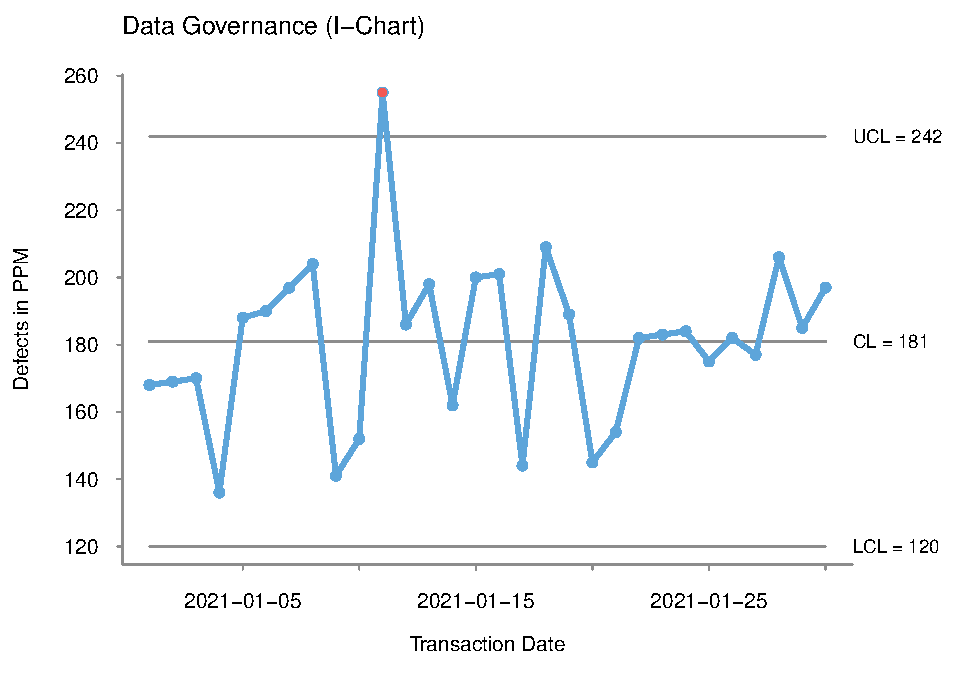
\includegraphics{_manage_MetadataGovernance_files/figure-latex/unnamed-chunk-2-1.pdf}

\hypertarget{summary}{%
\section{Summary}\label{summary}}

The above is just sample representation demonstrating a typical
monitoring mechanism for Metadata Governance information over daily
transactions. This information can be pulled for all parameters for all
databases across any given application. Using anomaly or defect
aggregation method the overall health score of data platforms can be
monitored and alerts sent if the health score / index degrades
significantly.

\end{document}
